\documentclass{standalone}
\usepackage{tikz}

\usetikzlibrary{shapes,arrows, backgrounds}
\begin{document}

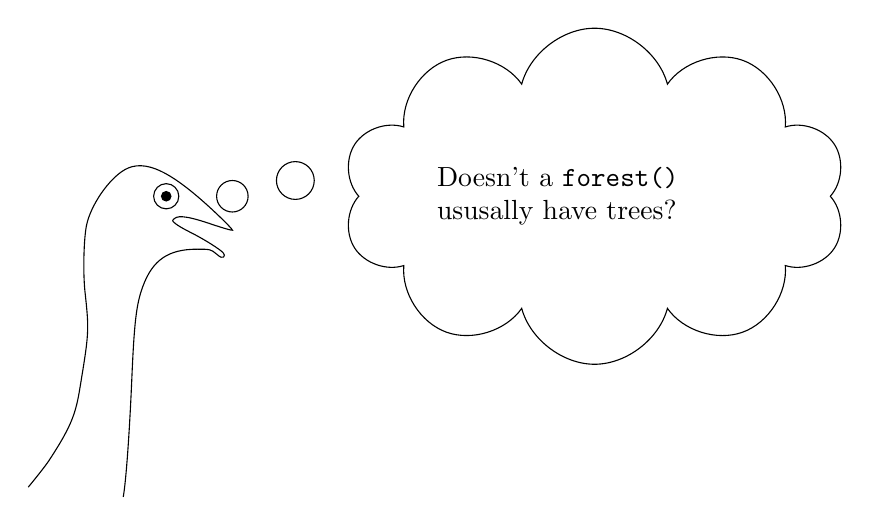
\begin{tikzpicture}[scale=0.2]

\begin{scope}%[xscale=-1]
%  draw EMU logo head
\draw  (150.38mm,-931.73mm)
% .. controls ++(5.77mm,11.57mm) and ++(-8.29mm,-9.98mm) .. ++(16.84mm,25.82mm)
.. controls ++(5.47mm,6.57mm) and ++(-1.72mm,-2.63mm) .. ++(13.07mm,16.74mm)
.. controls ++(13.10mm,20.00mm) and ++(-2.64mm,-15.96mm) .. ++(19.46mm,44.47mm)
.. controls ++(6.21mm,37.59mm) and ++(2.73mm,-25.43mm) .. ++(3.49mm,63.12mm)
.. controls ++(-1.29mm,12.06mm) and ++(-1.79mm,-8.49mm) .. ++(1.02mm,42.08mm)
.. controls ++(2.69mm,12.74mm) and ++(-10.07mm,-5.78mm) .. ++(24.20mm,35.14mm)
.. controls ++(12.77mm,7.34mm) and ++(-28.79mm,27.21mm) .. ++(58.36mm,-27.91mm)
.. controls ++(5.81mm,-5.49mm) and ++(0.28mm,0.27mm) .. ++(10.05mm,-10.47mm)
.. controls ++(-0.28mm,-0.27mm) and ++(6.69mm,-2.27mm) .. ++(-12.67mm,3.63mm)
.. controls ++(-14.48mm,4.92mm) and ++(2.76mm,2.09mm) .. ++(-23.92mm,3.92mm)
.. controls ++(-1.87mm,-1.42mm) and ++(-2.39mm,1.98mm) .. ++(0.54mm,-3.46mm)
.. controls ++(1.34mm,-1.11mm) and ++(-3.65mm,1.80mm) .. ++(9.07mm,-5.29mm)
.. controls ++(8.12mm,-4.01mm) and ++(-1.86mm,2.21mm) .. ++(21.09mm,-13.13mm)
.. controls ++(1.00mm,-1.19mm) and ++(0.79mm,0.77mm) .. ++(0.29mm,-2.69mm)
.. controls ++(-0.79mm,-0.77mm) and ++(2.56mm,-2.20mm) .. ++(-4.58mm,1.95mm)
.. controls ++(-3.37mm,2.90mm) and ++(8.38mm,-0.00mm) .. ++(-12.21mm,3.01mm)
.. controls ++(-18.37mm,-0.00mm) and ++(6.21mm,16.92mm) .. ++(-34.52mm,-23.75mm)
.. controls ++(-4.08mm,-11.11mm) and ++(1.56mm,36.30mm) .. ++(-6.96mm,-58.49mm)
.. controls ++(-1.52mm,-35.37mm) and ++(1.75mm,9.82mm) .. ++(-5.44mm,-75.07mm)
;
% eye
\draw (238.00mm,-747.00mm) circle (8mm);
\draw [fill=black](238.00mm,-747.00mm) circle (3mm);

% bubbles
\draw (280.00mm,-747.00mm) circle (10mm);
\draw (320.00mm,-737.00mm) circle (12mm);

\node[cloud, aspect=2, draw=black, text width=4cm] at (510.00mm,-747.00mm){Doesn't a \texttt{forest()} ususally have trees?};


\end{scope}



% \draw (600.00mm,-0.00mm) circle (20mm);

% \draw (500.00mm,-50.00mm) circle (30mm);

% \node[ellipse, draw, text width = 3cm] (into_a) at (-0.00mm, -200.00mm) {$\sqrt{-1} = i$};

\end{tikzpicture}

\end{document}
